\documentclass[a4paper,12pt]{report}
\usepackage{amssymb}

\usepackage{ucs}
\usepackage[utf8x]{inputenc} % Input encoding for Greek characters
\usepackage[greek,english]{babel} % Language support

\newcommand{\en}{\selectlanguage{english}}
\newcommand{\gr}{\selectlanguage{greek}}

% \usepackage{algorithm2e}
% \usepackage{algorithm}
% \usepackage{algorithmic}
\usepackage{enumitem}
\usepackage{tcolorbox}
\tcbuselibrary{listingsutf8}
\usepackage{float}
\usepackage{amsmath}
\usepackage{graphicx} % For including images
\usepackage{titlesec} % Custom title formatting
\usepackage{fancyhdr} % For custom headers and footers
\usepackage{geometry} % For adjusting page margins

% Adjust the page margins to make content wider
\geometry{top=2.5cm, bottom=2.5cm, left=2.5cm, right=2.5cm}

% Redefine chapter formatting to make it smaller
\titleformat{\chapter}[display]
    {\normalfont\LARGE\bfseries} % Smaller size and bold for chapter heading
    {\chaptername\ \thechapter} % Chapter number format
    {15pt} % Space between chapter number and title
    {\bfseries} % Smaller size and bold for chapter title
\begin{document}

\begin{titlepage}
    \centering
    \vspace*{-3cm}
    % University logo
    \includegraphics[width=1\textwidth]{auth_logo.png} % Replace with your actual logo file

    % University name in Greek
    \textbf{\gr ΑΡΙΣΤΟΤΕΛΕΙΟ ΠΑΝΕΠΙΣΤΗΜΙΟ ΘΕΣΣΑΛΟΝΙΚΗΣ}
    \vspace{2cm}

    % Document title and subtitle in Greek
    \LARGE\textbf{\gr Ψηφιακή Επεξεργασία Εικόνας Αναφορά} \\
    \Large\normalfont{\gr Εργασία 2} \\
    \vspace{4cm}

    \gr
    \large
    \textbf{Διακολουκάς Δημήτριος} \\
    \textbf{AEM 10642}
    \vspace{2.5cm}

    \en
    \textit{Email: ddiakolou@ece.auth.gr}
\end{titlepage}

\gr
\tableofcontents

\chapter{Εισαγωγή και περιγραφή εργασίας}

Η παρούσα εργασία εντάσσεται στο πλαίσιο του μαθήματος \textbf{Ψηφιακή Επεξεργασία Εικόνας} και έχει ως κύριο αντικείμενο την ανίχνευση ακμών και κυκλικών περιγραμμάτων σε εικόνες, μέσω τεχνικών \en convolution \gr και της μεθόδου \en Hough Transform\gr.

\vspace{0.3cm}

\hspace{-0.6cm}Πιο συγκεκριμένα, αξιοποιούνται και υλοποιούνται τα παρακάτω βασικά εργαλεία:

\begin{itemize}
    \item \textbf{\en FIR convolution\gr}, που χρησιμοποιείται ως βασική λειτουργία για τη δημιουργία φίλτρων στην επεξεργασία εικόνας.
    
    \item \textbf{Ανίχνευση ακμών με \en Sobel\gr}, για την εξαγωγή περιοχών έντονων μεταβολών φωτεινότητας με χρήση πρώτων παραγώγων.

    \item \textbf{Ανίχνευση ακμών με \en LoG (Laplacian of Gaussian)\gr}, που εφαρμόζει φίλτρο \en Gaussian \gr για εξομάλυνση και εντοπισμό ακμών μέσω της δεύτερης παραγώγου.

    \item \textbf{Ανίχνευση κύκλων με \en Hough Transform\gr}, όπου ανιχνεύονται κυκλικά σχήματα σε δυαδικές εικόνες μέσω ψηφοφορίας σε έναν τρισδιάστατο πίνακα (κέντρο $x$, $y$, ακτίνα $r$).
\end{itemize}

\vspace{0.3cm}

\hspace{-0.6cm}Η εργασία αποτελείται από:

\begin{enumerate}
    \item Συνάρτηση \en\texttt{fir\_conv()} \gr για συνέλιξη εικόνας με μάσκα.
    \item Συνάρτηση \en \texttt{sobel\_edge()} \gr για ανίχνευση ακμών με \en Sobel\gr.
    \item Συνάρτηση \en \texttt{log\_edge()} \gr για εντοπισμό ακμών μέσω \en zero-crossings \gr του φίλτρου \en LoG\gr.
    \item Συνάρτηση \en \texttt{circ\_hough()} \gr για εύρεση κύκλων σε εικόνες ακμών.
    \item Το αρχείο \en \texttt{demo.py}\gr, το οποίο συντονίζει την όλη ροή, εφαρμόζει τις παραπάνω συναρτήσεις στην εικόνα \en \texttt{basketball\_large.png} \gr η οποία παρουσιάζεται στο σχήμα παρακάτω και εξάγει τα τελικά αποτελέσματα.
\end{enumerate}

\begin{figure}[H]
\centering

\includegraphics[width=0.6\textwidth]{basketball_large.png}
\caption{Εικόνα μπάλας μπάσκετ που δίνεται από τα δεδομένα.}
\end{figure}

\vspace{0.3cm}

\hspace{-0.6cm}Σκοπός της εργασίας είναι η υλοποίηση αυτών των τεχνικών από το μηδέν, χωρίς έτοιμες βιβλιοθήκες \en edge detection \gr ή \en circle detection\gr, παρά μόνο με χρήση βασικών πακέτων της \en Python \gr όπως \en NumPy, SciPy, Matplotlib, PIL \gr και \en OpenCV\gr, όπου απαιτείται για την απεικόνιση.

\vspace{0.3cm}

\hspace{-0.6cm}Το τελικό αποτέλεσμα περιλαμβάνει τόσο τις υλοποιήσεις όσο και την απεικόνιση των ακμών και των κύκλων, μαζί με σχολιασμό για διαφορετικές παραμέτρους, όπως το κατώφλι ανίχνευσης, η ελάχιστη ψήφος για τον μετασχηματισμό \en Hough (\texttt{V\_min}) \gr και η ακτίνα κύκλων.

\chapter{Συνέλιξη εικόνας με \en FIR \gr φίλτρα }

Στο πρώτο μέρος της εργασίας ζητείται η υλοποίηση της δισδιάστατης συνέλιξης εικόνας με \en FIR (Finite Impulse Response) \gr φίλτρα. Τα \en FIR \gr φίλτρα είναι μάσκες με πεπερασμένη υποστήριξη, δηλαδή μη μηδενικές τιμές εντός ενός πεπερασμένου ορθογωνίου χωρίου. Όταν εφαρμόζονται πάνω σε εικόνες, οδηγούν σε έξοδο μέσω της πράξης συνέλιξης.

\vspace{0.3cm}

\hspace{-0.6cm}Η έξοδος $g(n_1,n_2)$ από τη συνέλιξη μιας εικόνας εισόδου $f(n_1,n_2)$ με μάσκα $h(k_1,k_2)$ δίνεται από την εξίσωση:

\[
g(n_1,n_2) = \sum_{k_1 = N_{1,\min}}^{N_{1,\max}} \sum_{k_2 = N_{2,\min}}^{N_{2,\max}} h(k_1, k_2) \cdot f(n_1 - k_1, n_2 - k_2)
\]

\hspace{-0.6cm}Η πράξη αυτή πραγματοποιεί φιλτράρισμα στην εικόνα $f$, με τη μάσκα $h$ να σκανάρει κάθε θέση της εικόνας και να υπολογίζει έναν νέο συνδυασμένο φωτεινότητας, βασισμένο στα γειτονικά pixels.

\vspace{0.3cm}

\hspace{-0.6cm}Στην παρούσα εργασία, η υλοποίηση πραγματοποιείται μέσω της συνάρτησης \en \texttt{fir\_conv()}\gr, η οποία λαμβάνει ως είσοδο:

\begin{itemize}
    \item Την εικόνα \en (\texttt{in\_img\_array}
    \gr) ως πίνακα \en NumPy \gr 2 διαστάσεων.
    \item Τη μάσκα συνέλιξης \en (\texttt{h})\gr, επίσης ως \en 2D\gr πίνακα.
    \item Προαιρετικά την αρχή \en (\texttt{origin}\gr) της εικόνας και της μάσκας, ώστε να διατηρείται η σωστή αναφορά θέσης στο αποτέλεσμα.
\end{itemize}

Η συνάρτηση επιστρέφει:
\begin{itemize}
    \item Τον πίνακα εξόδου (πλήρους συνέλιξης) με διαστάσεις \en \texttt{(M+P-1, N+Q-1)}\gr.
    \item Τη θέση της αρχής $(0,0)$ στον πίνακα εξόδου.
\end{itemize}

\vspace{0.3cm}

\section*{Ανάλυση υλοποίησης}

Η υλοποίηση ακολουθεί πιστά τα μαθηματικά βήματα της συνέλιξης. Περιλαμβάνει αναστροφή της μάσκας, μηδενική επέκταση της εικόνας, και αθροιστικό πολλαπλασιασμό κατά στοιχείο μεταξύ μάσκας και τοπικής περιοχής της εικόνας.

\vspace{0.3cm}

\begin{tcolorbox}[colback=gray!5!white, colframe=black!75!black, title=Ανάλυση υλοποίησης \en \texttt{fir\_conv()}\gr]
\begin{itemize}
    \item Αρχικά γίνεται έλεγχος ότι τόσο η είσοδος όσο και η μάσκα είναι δισδιάστατοι πίνακες.

    \item Αν δεν δοθεί \en \texttt{in\_origin}\gr, θεωρείται ότι το $(0,0)$ της εισόδου βρίσκεται στην πάνω αριστερή γωνία. Αντίστοιχα, αν δεν δοθεί \en \texttt{mask\_origin}\gr, ορίζεται στο κέντρο της μάσκας.

    \item Η μάσκα $h$ αντιστρέφεται πλήρως και στους δύο άξονες (δηλαδή περιστρέφεται κατά 180 μοίρες), ώστε να ικανοποιεί τον μαθηματικό ορισμό της συνέλιξης.

    \item Η είσοδος $f$ επεκτείνεται με μηδενικά γύρω από την εικόνα \en (zero-padding)\gr, ώστε να μπορεί να μετακινηθεί πλήρως η μάσκα χωρίς απώλειες στα όρια.

    \item Αρχικοποιείται πίνακας εξόδου διαστάσεων \en \texttt{(M + P - 1, N + Q - 1)} \gr γεμάτος με μηδενικά.

    \item Για κάθε θέση $(i,j)$ στην εικόνα εξόδου:
    \begin{itemize}
        \item Επιλέγεται περιοχή από την επεκταμένη εικόνα, ίδιου μεγέθους με τη μάσκα.
        \item Υπολογίζεται το γινόμενο κατά στοιχείο με τη μάσκα που έχει ήδη αντιστραφεί.
        \item Αθροίζεται το αποτέλεσμα και αποθηκεύεται στη θέση $(i,j)$.
    \end{itemize}

    \item Τέλος, υπολογίζεται η νέα θέση του $(0,0)$ στην εικόνα εξόδου ως \en \texttt{in\_origin + mask\_origin}\gr.
\end{itemize}
\end{tcolorbox}

\vspace{0.3cm}

\section*{Παρατηρήσεις}

\begin{itemize}
    \item Η υλοποίηση είναι πλήρους συνέλιξης \en (full convolution) \gr και όχι έγκυρης \en (valid)\gr, δηλαδή επιστρέφει όλα τα πιθανά σημεία εφαρμογής της μάσκας, ακόμη και στα όρια της εικόνας.
    
    \item Η χρήση μηδενικού \en padding \gr επηρεάζει τις ακραίες περιοχές, αλλά είναι απαραίτητη για τη σωστή ευθυγράμμιση της μάσκας σε όλο το φάσμα της εικόνας.

    \item Η προαιρετική χρήση μεταβλητών \en \texttt{in\_origin} \gr και \en \texttt{mask\_origin} \gr επιτρέπει διατήρηση της πληροφορίας θέσης, χρήσιμο σε πιο σύνθετες εφαρμογές (π.χ. \en Hough Transform\gr).
\end{itemize}

\hspace{-0.6cm}H συνάρτηση υλοποιέιται με χρήση σχολίων στο αρχείο \en fir\_conv.py \gr και ονομάζεται \en fir\_conv()\gr.

\chapter{Ανίχνευση ακμών με τελεστή \en Sobel\gr}

Ο τελεστής \en Sobel \gr είναι ένας κλασικός γραμμικός τελεστής για την ανίχνευση ακμών, ο οποίος προσεγγίζει τις παραγώγους πρώτης τάξης κατά τις δύο χωρικές κατευθύνσεις $x_1$ και $x_2$ μέσω συνέλιξης της εικόνας με δύο προκαθορισμένες μάσκες διαστάσεων $3 \times 3$.

\vspace{0.3cm}

\hspace{-0.6cm}Οι δύο μάσκες \en Sobel \gr έχουν τη μορφή:

\[
G_{x_1} =
\begin{bmatrix}
-1 & 0 & +1 \\
-2 & 0 & +2 \\
-1 & 0 & +1
\end{bmatrix},
\quad
G_{x_2} =
\begin{bmatrix}
+1 & +2 & +1 \\
0  & 0  & 0  \\
-1 & -2 & -1
\end{bmatrix}
\]

\hspace{-0.6cm}Αυτές εφαρμόζονται στην εικόνα μέσω συνέλιξης για την προσέγγιση των παραγώγων κατά $x_1$ και $x_2$. Το τελικό μέτρο της κλίσης (ένταση της ακμής) υπολογίζεται ως:

\[
g(n_1, n_2) = \sqrt{g_1(n_1, n_2)^2 + g_2(n_1, n_2)^2}
\]

\hspace{-0.6cm}όπου $g_1$ και $g_2$ είναι οι εικόνες που προκύπτουν από τη συνέλιξη με τις μάσκες $G_{x_1}$ και $G_{x_2}$ αντίστοιχα. Τα σημεία όπου η $g(n_1,n_2)$ είναι υψηλή αντιστοιχούν σε ακμές στην εικόνα.

\vspace{0.3cm}

\hspace{-0.6cm}Η υλοποίηση της μεθόδου \en Sobel \gr πραγματοποιείται μέσω της συνάρτησης \en \texttt{sobel\_edge()}\gr, η οποία επιστρέφει ένα δυαδικό χάρτη ακμών για δεδομένο κατώφλι τιμής μεγέθους παραγώγου.

\vspace{0.3cm}

\section*{Ψευδοκώδικας υλοποίησης}

\begin{tcolorbox}[colback=gray!5!white, colframe=black!75!black, title=Ψευδοκώδικας \en sobel\_edge()\gr]
\en
\begin{verbatim}
1. Gx ← array [-1 0 +1; -2 0 +2; -1 0 +1]
   Gy ← array [+1 +2 +1; 0 0 0; -1 -2 -1]

2. mask_origin ← (1,1)
   in_origin ← (0,0)

3. [conv_x, origin_x]←fir_conv(in_img_array,Gx,in_origin,mask_origin)
   From conv_x extract:
     start_r, start_c ← origin_x
     end_r ← start_r + input_rows
     end_c ← start_c + input_cols
     gx ← conv_x[start_r:end_r, start_c:end_c]

4. Similarly for Gy:
   [conv_y, origin_y] ← fir_conv(...)
   gy ← cropped output as above

5. grad_mag ← sqrt(gx^2 + gy^2)

6. out_img_array ← same shape as input
   out_img_array ← (grad_mag ≥ thres)

7. return out_img_array
\end{verbatim}
\gr
\end{tcolorbox}

\vspace{0.3cm}

\section*{Ανάλυση υλοποίησης}

\begin{itemize}
    \item Οι μάσκες \en \texttt{Gx} \gr και \en \texttt{Gy} \grεφαρμόζονται με τη συνάρτηση \en \texttt{fir\_conv()} \gr που αναλύσαμε παραπάνω για απόλυτο έλεγχο στη θέση της αρχής.

    \item Το αποτέλεσμα της συνέλιξης είναι εικόνες ίδιων διαστάσεων με την είσοδο, καθώς γίνεται κατάλληλη αποκοπή (\en cropping \gr) από την πλήρη έξοδο, με βάση τη θέση της αρχής \en (\texttt{origin})\gr.

    \item Η ένταση ακμής προκύπτει ως \(\sqrt{g_x^2 + g_y^2}\).

    \item Τέλος, εφαρμόζεται κατώφλι \en (\texttt{thres}\gr) για να παραχθεί δυαδική εικόνα: \texttt{1} για έντονες ακμές, \texttt{0} αλλιώς.
\end{itemize}

\vspace{0.3cm}

\begin{tcolorbox}[colback=gray!5!white, colframe=black!75!black, title=Παρατήρηση]
Ο τελεστής \en Sobel \gr είναι ιδιαίτερα χρήσιμος καθώς ενσωματώνει φιλτράρισμα τύπου \en Gaussian smoothing \gr (μέσω των τιμών [1,2,1]) με αριθμητική παράγωγο. Έτσι, μειώνεται ο θόρυβος και ενισχύονται οι πραγματικές ακμές.
\end{tcolorbox}

\hspace{-0.6cm}Η αντίστοιχη υλοποίηση με σχολιασμό βρίσκεται στο αρχείο \en sobel\_edge.py \gr και συγκεκριμένα η υλοποίηση στην συνάρτηση \en sobel\_edge()\gr.

\section*{Αποτελέσματα και συμπεράσματα \en Sobel \gr}

Στο αρχείο εκτέλεσης \en demo.py \gr αφού γίνει η φόρτωση της εικόνας \en basketball\_large.py \gr και η μετατροπή της θεωρητικά σε \en float32 array \gr σε \en [0,1] format \gr(\(np.ndarray\)) ακολουθέι η κλήση της συνάρτησης \en sobel\_edge(...) \gr υπό καθορισμένες παραμέτρους κλήσεως \en threshold \gr και βεβαίως \(grayscale\) εικόνας. Έπειτα τα αποτελέσματα ο κώδικας τα αποθηκεύει σε \en .png \gr μορφή για οπτικοποίηση.

\subsection*{\en Output Sobel \gr για διάφορα \en thresholds \gr}

Παρακάτω παρατίθενται τα αντίστοιχα σχήματα που προέκυψαν από την κλήση της συνάρτησης \en sobel\_edge().\gr

\begin{figure}[H]
\centering

\begin{minipage}{0.48\textwidth}
    \centering
    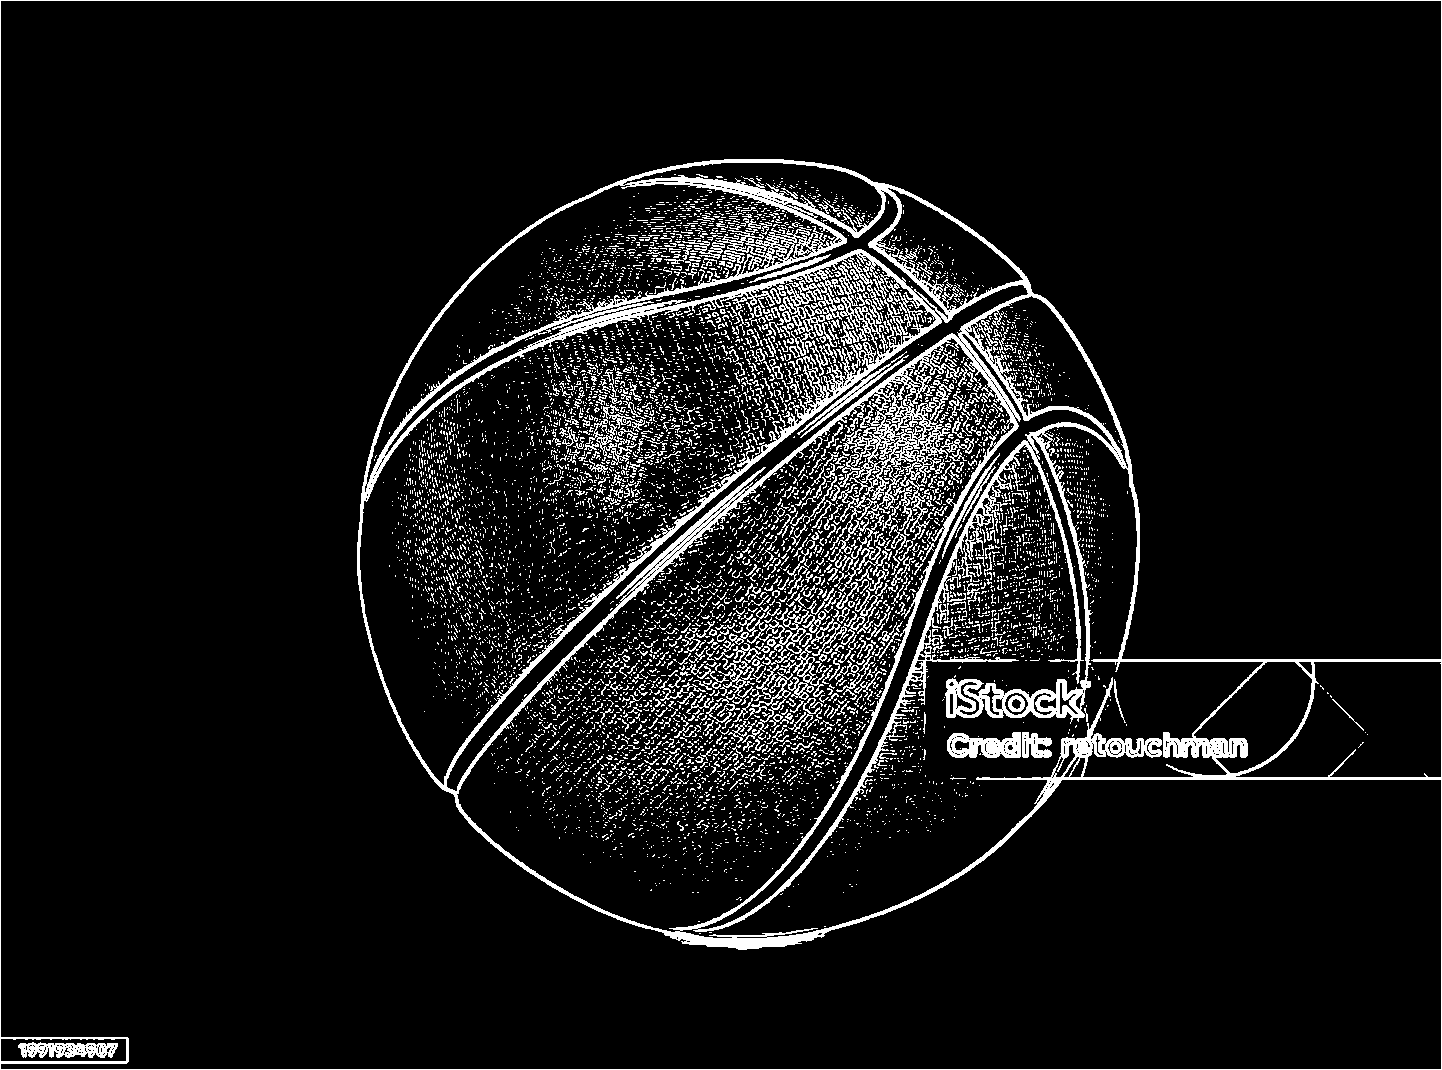
\includegraphics[width=\linewidth]{sobel.png}
    \caption{Εικόνα μπάλας μπάσκετ με εφαρμογή \en sobel \gr και \en threshold \gr 0.25.}
\end{minipage}
\hfill
\begin{minipage}{0.48\textwidth}
    \centering
    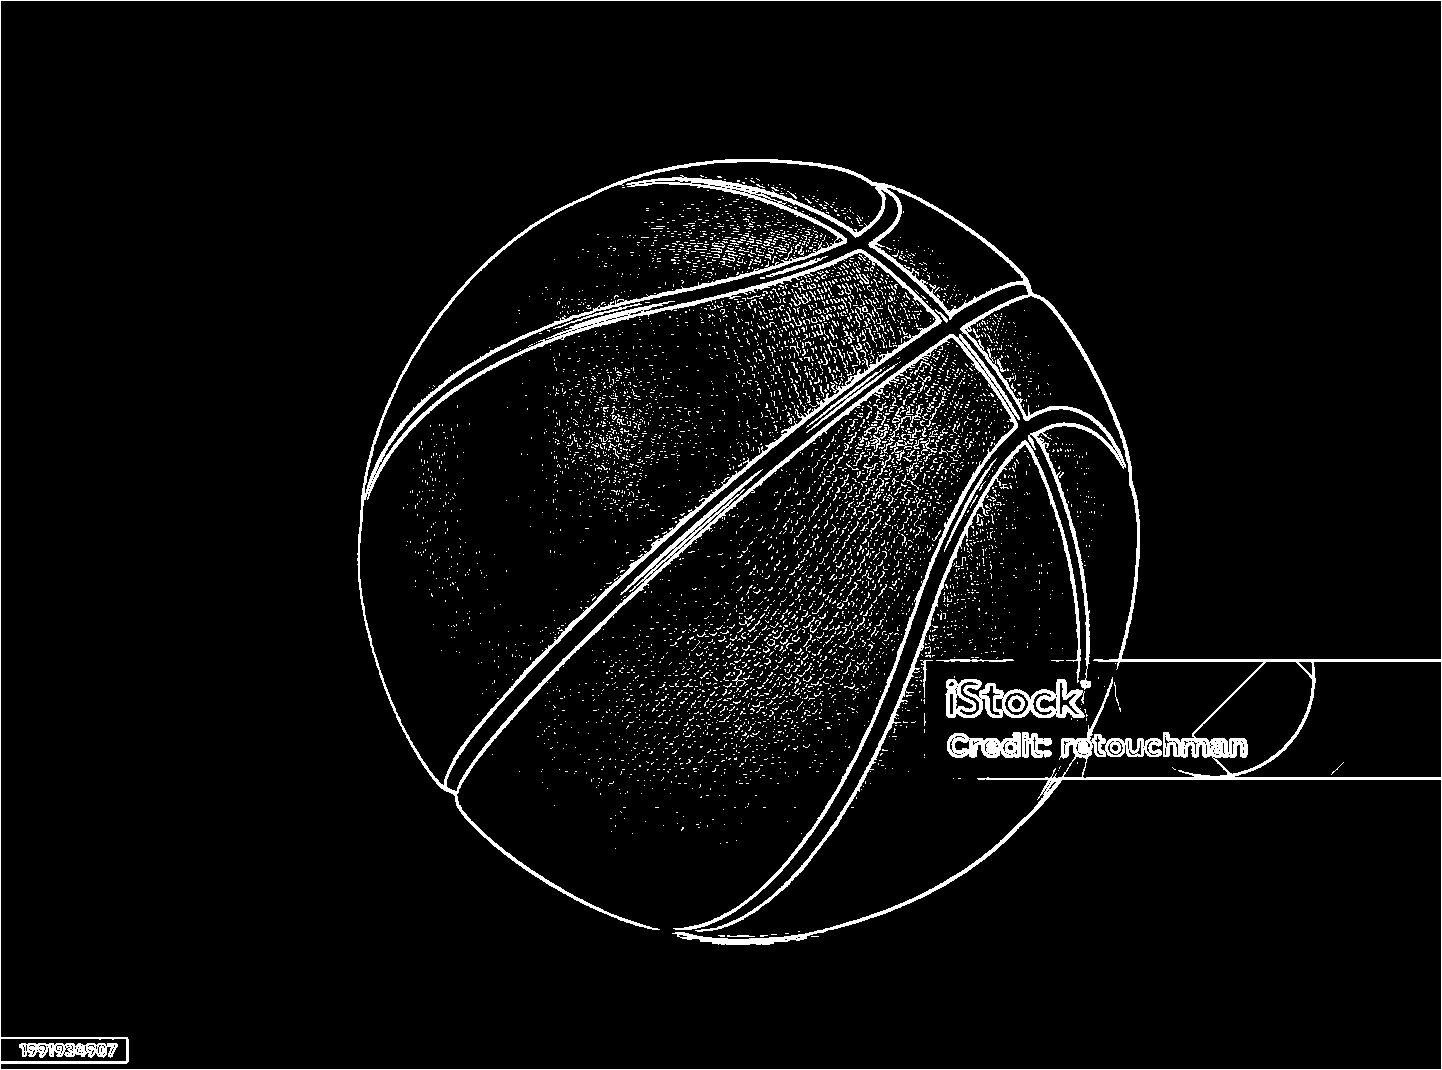
\includegraphics[width=\linewidth]{sobel_0_33.png}
    \caption{Εικόνα μπάλας μπάσκετ με εφαρμογή \en sobel \gr και \en threshold \gr 0.33.}
\end{minipage}

\end{figure}

\begin{figure}[H]
\centering

\begin{minipage}{0.48\textwidth}
    \centering
    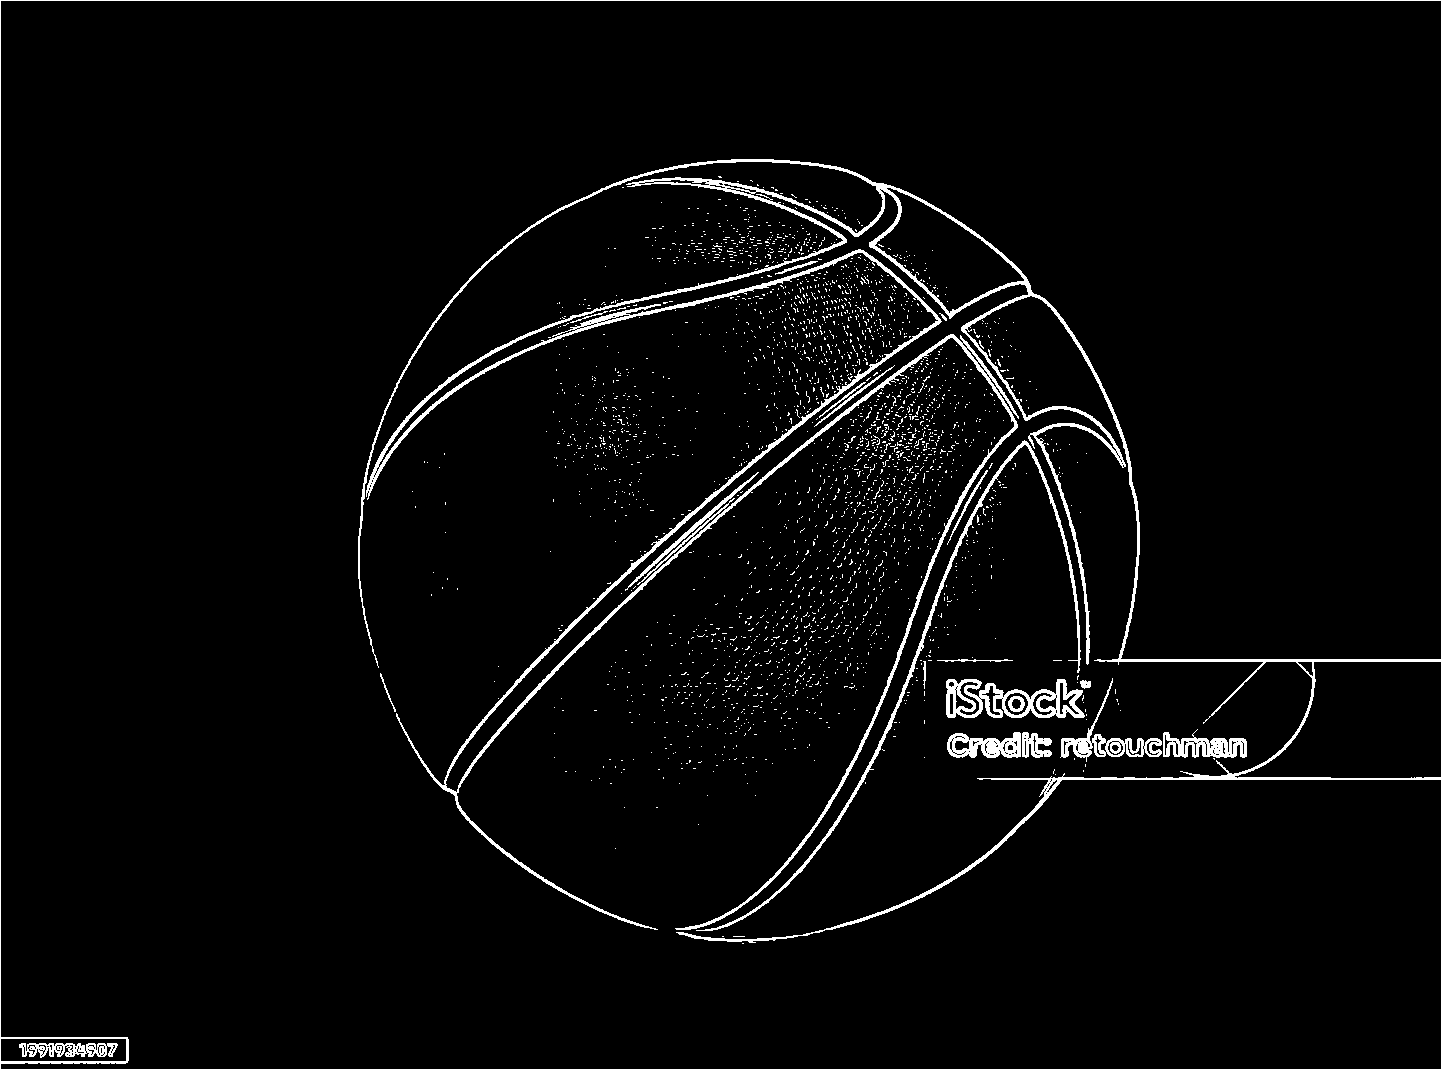
\includegraphics[width=\linewidth]{sobel_0_4.png}
    \caption{Εικόνα μπάλας μπάσκετ με εφαρμογή \en sobel \gr και \en threshold \gr 0.4.}
\end{minipage}
\hfill
\begin{minipage}{0.48\textwidth}
    \centering
    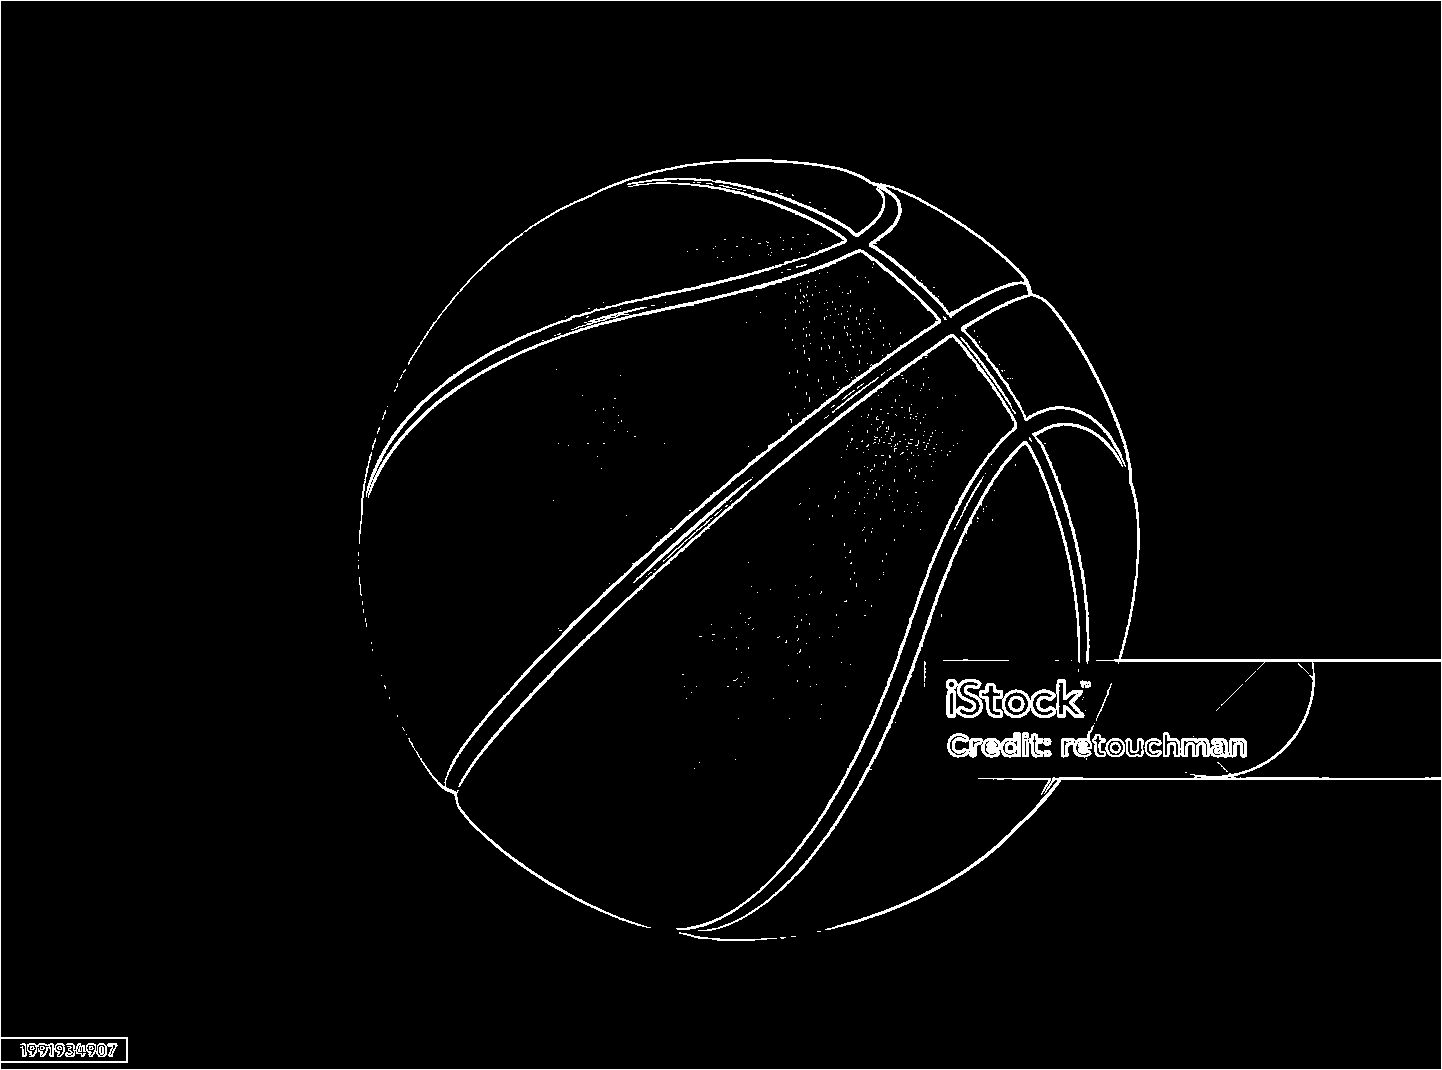
\includegraphics[width=\linewidth]{sobel_0_5.png}
    \caption{Εικόνα μπάλας μπάσκετ με εφαρμογή \en sobel \gr και \en threshold \gr 0.5.}
\end{minipage}

\end{figure}

\subsection*{Συμπεράσματα για διαφορετικές τιμές \en \texttt{threshold} \gr στον τελεστή \en Sobel\gr}

Για την αξιολόγηση της ευαισθησίας του τελεστή \en Sobel \gr ως προς την παράμετρο κατωφλίου, εφαρμόστηκε η συνάρτηση \en \texttt{sobel\_edge()} \gr σε διαφορετικές τιμές του \en \texttt{threshold}\gr. Η έξοδος είναι ένας δυαδικός χάρτης ακμών που εξαρτάται άμεσα από το πόσο έντονη πρέπει να είναι η κλίση ώστε να θεωρηθεί ακμή.

\vspace{0.3cm}

\hspace{-0.6cm}Παρατηρήσεις από τα αποτελέσματα:

\begin{itemize}
    \item Για \en \textbf{sobel\_thres = 0.25}\gr, οι ακμές είναι πιο πυκνές και ανιχνεύονται ακόμα και περιοχές με μέτριες μεταβολές στη φωτεινότητα. Αυτό μπορεί να περιλαμβάνει και θόρυβο ή ανεπιθύμητες λεπτομέρειες.
    
    \item Για \en \textbf{sobel\_thres = 0.33}\gr, η εικόνα παρουσιάζει λιγότερες ακμές, καθώς απορρίπτονται πιο αδύναμες κλίσεις. Η περιγραφή του κυρίου αντικειμένου (η μπάλα) παραμένει ικανοποιητική.

    \item Με τιμές όπως \en \textbf{sobel\_thres = 0.4} \gr και \textbf{0.5}, η ανίχνευση επικεντρώνεται πλέον στις ισχυρότερες ακμές της εικόνας, κυρίως στο περίγραμμα της μπάλας και στις εσωτερικές καμπύλες. Ωστόσο, λεπτομέρειες μικρής έντασης παραλείπονται.
\end{itemize}

\vspace{0.2cm}

\hspace{-0.6cm}Η επιλογή της τιμής \en \texttt{threshold} \gr επηρεάζει σημαντικά την πληρότητα και την ακρίβεια της ανίχνευσης. Χαμηλές τιμές οδηγούν σε υπερανίχνευση, ενώ υψηλές ενδέχεται να παραλείψουν χρήσιμες πληροφορίες. Η κατάλληλη ρύθμιση εξαρτάται από την εφαρμογή.

\chapter{Ανίχνευση ακμών με τελεστή \en Laplacian of Gaussian (LoG)\gr}

Ο τελεστής \en Laplacian of Gaussian (LoG) \gr χρησιμοποιείται για την ανίχνευση ακμών, εντοπίζοντας σημεία της εικόνας όπου η δεύτερη παράγωγος της έντασης αλλάζει πρόσημο — τα λεγόμενα \en zero crossings\gr. Η διαδικασία περιλαμβάνει δύο στάδια:

\begin{itemize}
    \item Εξομάλυνση της εικόνας με δισδιάστατο \en Gaussian \gr πυρήνα (για απομάκρυνση θορύβου).
    \item Εφαρμογή της \en Laplacian \gr στον εξομαλυμένο πυρήνα, ώστε να εντοπιστούν περιοχές υψηλής καμπυλότητας.
\end{itemize}

\vspace{0.3cm}

\section*{Μαθηματικό υπόβαθρο}

Ο πυρήνας \en LoG \gr προκύπτει από την εξίσωση:

\[LoG(x_1, x_2) = -\frac{1}{\pi \sigma^4} \left(1 - \frac{x_1^2 + x_2^2}{2\sigma^2}\right) e^{-\frac{x_1^2 + x_2^2}{2\sigma^2}}
\]

\hspace{-0.6cm}Η εικόνα υφίσταται συνέλιξη με αυτό τον πυρήνα και οι ακμές ανιχνεύονται εντοπίζοντας αλλαγές πρόσημου (δηλαδή σημεία όπου η τιμή αλλάζει από θετική σε αρνητική ή το αντίστροφο).

\vspace{0.3cm}

\section*{Υλοποίηση \en \texttt{\_generate\_log\_kernel()}\gr}

Η συνάρτηση δημιουργεί διακριτό \en LoG \gr πυρήνα με βάση το \(\sigma\) και την εξίσωση που παρέθεσα πιο πάνω. Η περιοχή υπολογισμού είναι \([-3\sigma, 3\sigma]\), που καλύπτει την πλειοψηφία της Γκαουσιανής.

\begin{tcolorbox}[colback=gray!5!white, colframe=black!75!black, title=Ψευδοκώδικας \en \_generate\_log\_kernel()\gr]
\en
\begin{verbatim}
1. k ← ceil(3 * sigma)
2. x1, x2 ← [-k, ..., k]
3. X1, X2 ← meshgrid(x1, x2)

4. r_squared ← X1^2 + X2^2
5. factor ← -1 / (pi * sigma^4)
6. log_kernel ← factor * (1 - r_squared / (2*sigma^2)) *
                            exp(-r_squared / (2*sigma^2))

7. Return log_kernel and origin = (k, k)
\end{verbatim}
\gr
\end{tcolorbox}

\vspace{0.3cm}

\section*{Υλοποίηση \en \texttt{\_zero\_crossings()}\gr}

Η συνάρτηση ελέγχει σε κάθε σημείο (εκτός ορίων) αν η τοπική περιοχή \(3\times3\) περιέχει τιμές τόσο θετικές όσο και αρνητικές — ένδειξη μηδενικής διέλευσης.

\begin{tcolorbox}[colback=gray!5!white, colframe=black!75!black, title=Ψευδοκώδικας \en \_zero\_crossings()\gr]
\en
\begin{verbatim}
1. Initialize output as zero array (same shape as input)

2. For each pixel (r, c) excluding borders:
   - patch ← 3x3 region centered at (r, c)
   - If patch.min() < 0 and patch.max() > 0:
       → output[r, c] ← 1 (edge detected)

3. Return output
\end{verbatim}
\gr
\end{tcolorbox}

\vspace{0.3cm}

\section*{Υλοποίηση \en \texttt{log\_edge()}\gr}

Αυτή είναι η κύρια συνάρτηση. Παράγει τον \en LoG \gr πυρήνα, εφαρμόζει συνέλιξη μέσω \en \texttt{fir\_conv()}\gr, κάνει κατάλληλο \en \texttt{cropping} \gr και εντοπίζει ακμές μέσω \en \texttt{zero-crossings}\gr.

\begin{tcolorbox}[colback=gray!5!white, colframe=black!75!black, title=Ψευδοκώδικας \en log\_edge()\gr]
\en
\begin{verbatim}
1. h_log, mask_origin ← _generate_log_kernel(sigma)

2. conv_full, out_origin ← fir_conv(
       in_img_array, h_log,
       in_origin = (0,0),
       mask_origin = mask_origin
   )

3. Crop result from conv_full using out_origin:
   log_img ← conv_full[r0:r1, c0:c1]

4. result ← _zero_crossings(log_img)

5. Return result
\end{verbatim}
\gr
\end{tcolorbox}

\vspace{0.3cm}

\section*{Παραγόμενη εικόνα εξόδου \en LoG \gr και ανάλυση αποτελεσμάτων}

Με παρόμοιο τρόπο με την μέθοδο \en Sobel \gr έτσι και στην μέθοδο \en LoG \gr κλήθηκε η συνάρτηση \en log\_edge(...) \gr υπό καθορισμένες παραμέτρους κλήσεως (\(σ = 1\)) και βεβαίως \(grayscale\) εικόνας. Έπειτα τα αποτελέσματα ο κώδικας τα αποθηκεύει σε \en .png \gr μορφή για οπτικοποίηση.

\begin{figure}[H]
\centering
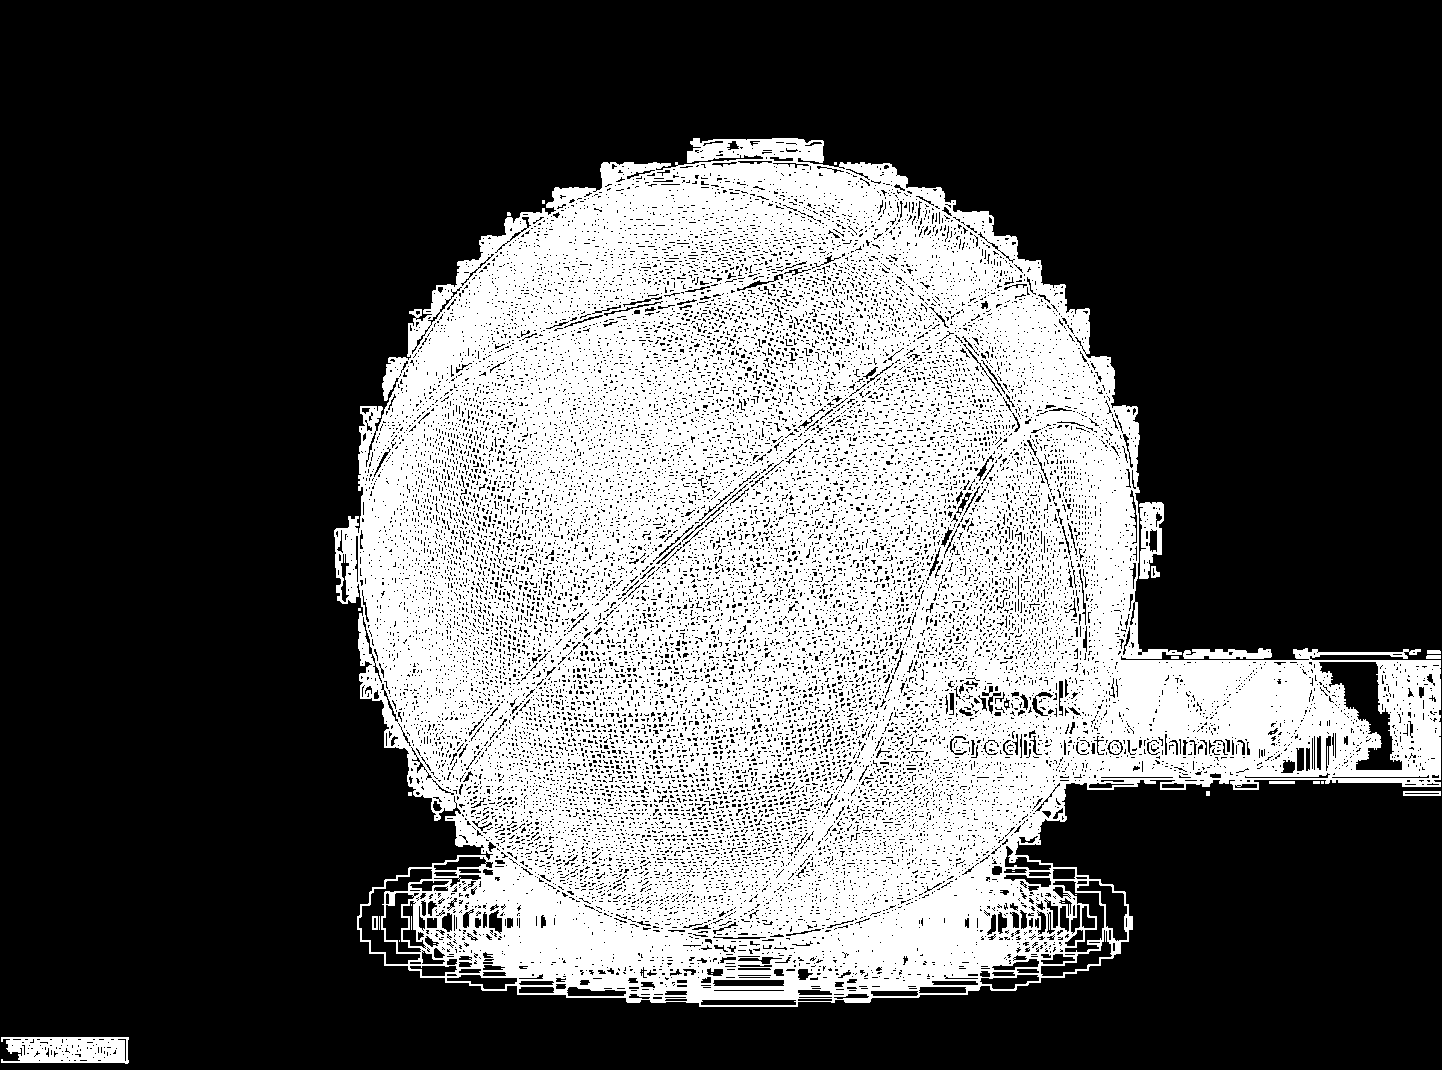
\includegraphics[width=0.6\textwidth]{log.png}
\caption{Ανίχνευση ακμών με τελεστή \en LoG \gr για \(\sigma = 1.0\). Οι ακμές εντοπίζονται στα σημεία μηδενικής διέλευσης.}
\end{figure}

\subsection*{Παρατηρήσεις και συμπεράσματα \en LoG \gr και σύγκριση με \en Sobel\gr}

Έτσι, λοιπόν, παραθέτω παρακάτω και ορισμένες από τις διαπιστώσεις μου για την εφαρμογή της μεθόδου \en LoG \gr συγκριτικά και με την μέθοδο \en Sobel \gr.

\begin{itemize}
    \item Η έξοδος του \en LoG \gr είναι πιο συνεχής σε σχέση με τον \en Sobel\gr, αναδεικνύοντας περιοχές με καμπυλότητες και διαφορές φωτεινότητας, ακόμη κι αν δεν αποτελούν έντονες ακμές.

    \item Το αποτέλεσμα περιλαμβάνει πολλές λεπτές γραμμές, καθώς εντοπίζονται μηδενικές διελεύσεις ακόμη και σε ήπιες μεταβολές — χαρακτηριστικό της δεύτερης παραγώγου.

    \item Παρότι η εξομάλυνση με \(\sigma = 1.0\) μειώνει τον θόρυβο, εξακολουθούν να εμφανίζονται εσωτερικές υφές και δομές στην επιφάνεια της μπάλας.

    \item Σε σύγκριση με τον \en Sobel\gr, το \en LoG \gr αποφεύγει την ανάγκη ορισμού κατωφλίου, ωστόσο παράγει πιο πολύπλοκη έξοδο που περιλαμβάνει και ακμές «χαμηλής έντασης» (εντός του αντικειμένου).
    
    \item Η μέθοδος είναι χρήσιμη όταν επιθυμούμε πλήρη ανάδειξη δομών και όχι μόνο των πιο ισχυρών ακμών (όπως κάνει ο \en Sobel \gr με κατάλληλο \en threshold\gr).
\end{itemize}

\hspace{-0.6cm}Ο αντίστοιχος κώδικας για την υλοποίηση της μεθόδου \en LoG \gr βρίσκεται στο αρχείο \en log\_edge.py \gr και η συνάρτηση κλήσεως είναι η \en log\_edge()\gr.


\chapter{Ανίχνευση κύκλων με μετασχηματισμό \en Hough\gr}

Ο μετασχηματισμός \en Hough \gr αποτελεί μία κλασική παραμετρική μέθοδο για την ανίχνευση καμπυλών, όπως ευθείες, κύκλοι και έλλειψης. Στην παρούσα εργασία εστιάζουμε στην ανίχνευση κυκλικών περιγραμμάτων (π.χ. μπάλας) μέσω ενός τρισδιάστατου παραμετρικού χώρου \((x, y, r)\), όπου \(x,y\) είναι τα κέντρα και \(r\) η ακτίνα κάθε υποψήφιου κύκλου.

\vspace{0.3cm}

\section*{Αρχή μεθόδου}

Για κάθε στοιχείο ακμής \((x_i, y_i)\) που προκύπτει από τεχνικές ανίχνευσης ακμών (\en Sobel \gr ή \en LoG\gr), η μέθοδος:

\begin{itemize}
    \item Εξετάζει όλους τους δυνατούς κύκλους που θα μπορούσαν να περνούν από το σημείο αυτό.
    \item Υποθέτει διαφορετικές ακτίνες και γωνίες, και «ψηφίζει» για τα κέντρα αυτών των κύκλων στον χώρο παραμέτρων.
    \item Οι κύκλοι με υψηλό πλήθος ψήφων θεωρούνται ανιχνευμένοι.
\end{itemize}

\hspace{-0.6cm}Η ψήφιση γίνεται σε έναν \en \textbf{accumulator} \gr και οι κύκλοι εξάγονται είτε μέσω ορίου ψήφων (\en V\_min\gr) είτε μέσω ταξινόμησης κατά ψήφους.

\vspace{0.3cm}

\section*{Βελτιστοποίηση μνήμης και απόδοσης}

Η πλήρης σάρωση σε εικόνα υψηλής ανάλυσης μπορεί να οδηγήσει σε:

\begin{itemize}
    \item \textbf{Υπερβολική κατανάλωση μνήμης}, λόγω του πλήθους των πιθανών συνδυασμών \((x, y, r)\) \en (Message \gr \textbf{\en killed \gr}στο \en terminal\gr).
    \item \textbf{Χρόνο εκτέλεσης} απαγορευτικό για διαδραστικές εφαρμογές και διαρκές \(testing\) για επιδίωξη βέλτιστων αποτελεσμάτων.
\end{itemize}

\hspace{-0.6cm}Για τον λόγο αυτό χρησιμοποιήθηκε η βοηθητική συνάρτηση \en \texttt{resize\_custom\_func()}\gr, η οποία μειώνει το μέγεθος της εικόνας κατά 4 φορές, περιορίζοντας έτσι σημαντικά τις απαιτήσεις.

\begin{tcolorbox}[colback=gray!5!white, colframe=black!75!black, title=Ψευδοκώδικας \en resize\_custom\_func()\gr]
\en
\begin{verbatim}
1. Load image from "name.png"
2. Compute new shape ← (H/4, W/4)
3. Apply resizing with anti_aliasing and preserve range
4. Save new image as "name_small.png"
\end{verbatim}
\gr
\end{tcolorbox}

\hspace{-0.6cm}Παρακάτω παρατίθενται και οι εικόνες μειωμένου μεγέθους \en pixels \gr πριν και μετά την χρήση της συνάρτησης για να δειχθεί ακριβώς τι εικόνα χρησιμοποιήθηκε για την συνάρτηση \en circ\_hough() \gr.

\begin{figure}[H]
\centering

\begin{minipage}{0.48\textwidth}
    \centering
    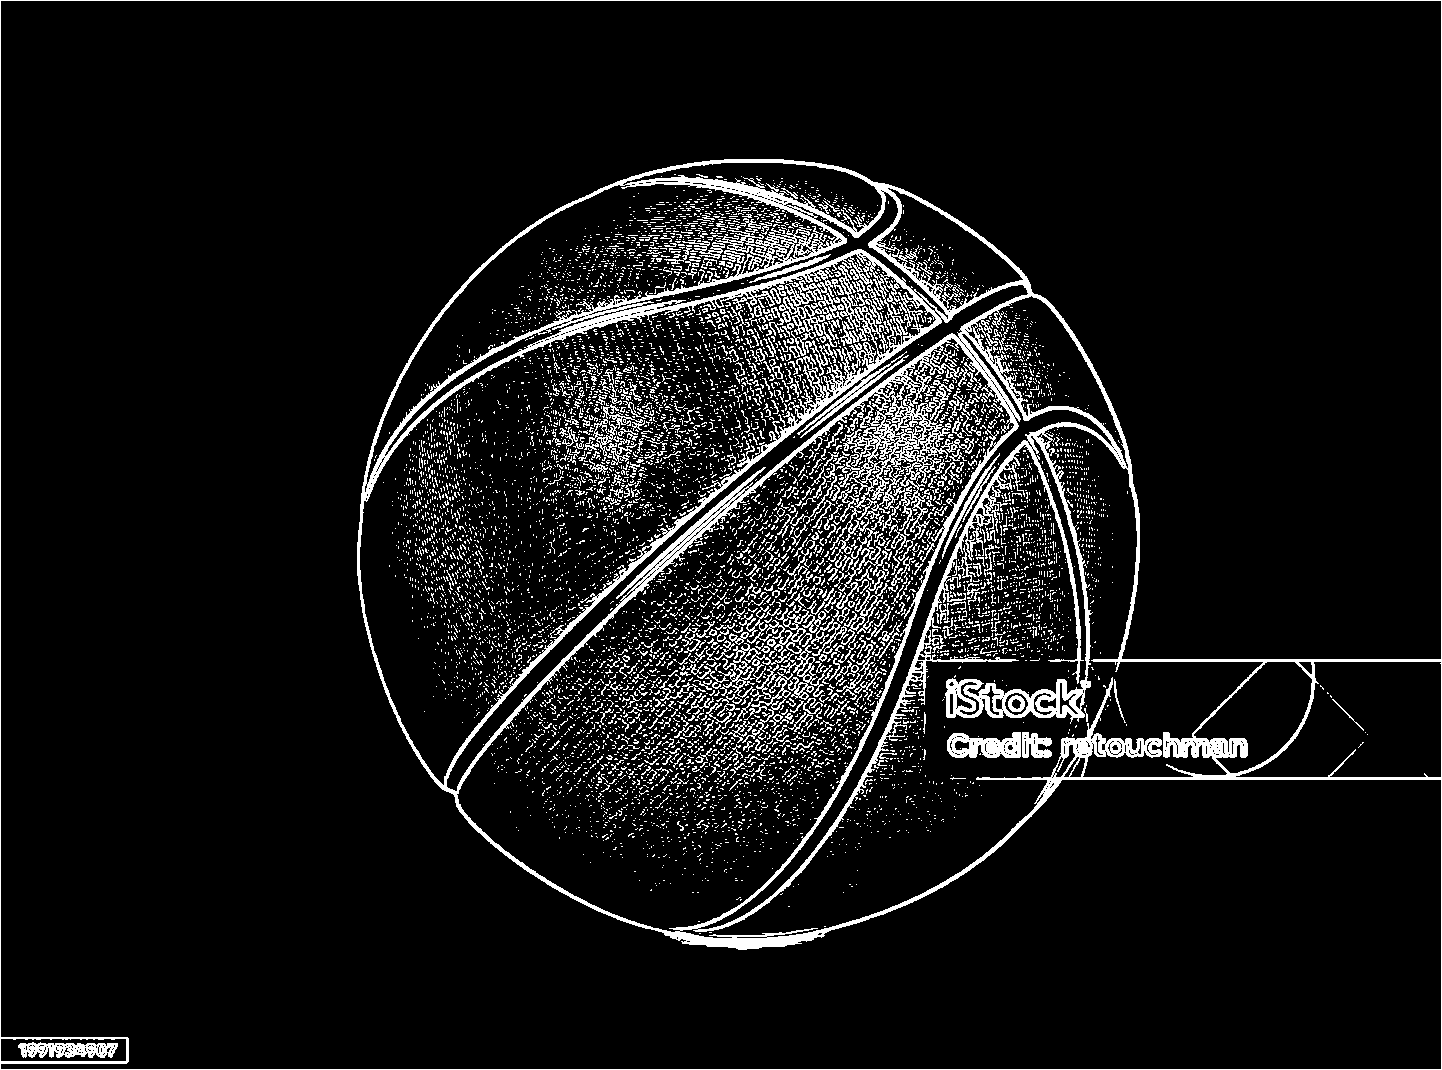
\includegraphics[width=\linewidth]{sobel.png}
    \caption{Εικόνα μπάλας μπάσκετ με εφαρμογή \en sobel \gr και \en threshold \gr 0.25.}
\end{minipage}
\hfill
\begin{minipage}{0.48\textwidth}
    \centering
    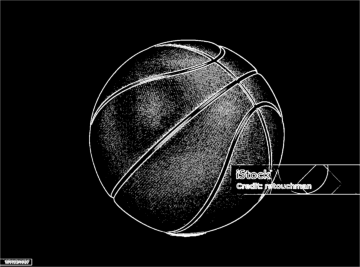
\includegraphics[width=\linewidth]{sobel_small.png}
    \caption{Εικόνα μπάλας μπάσκετ με εφαρμογή \en sobel \gr και \en threshold \gr 0.25 μειωμένης διάστασης \en pixel\gr.}
\end{minipage}

\end{figure}

\begin{figure}[H]
\centering

\begin{minipage}{0.48\textwidth}
    \centering
    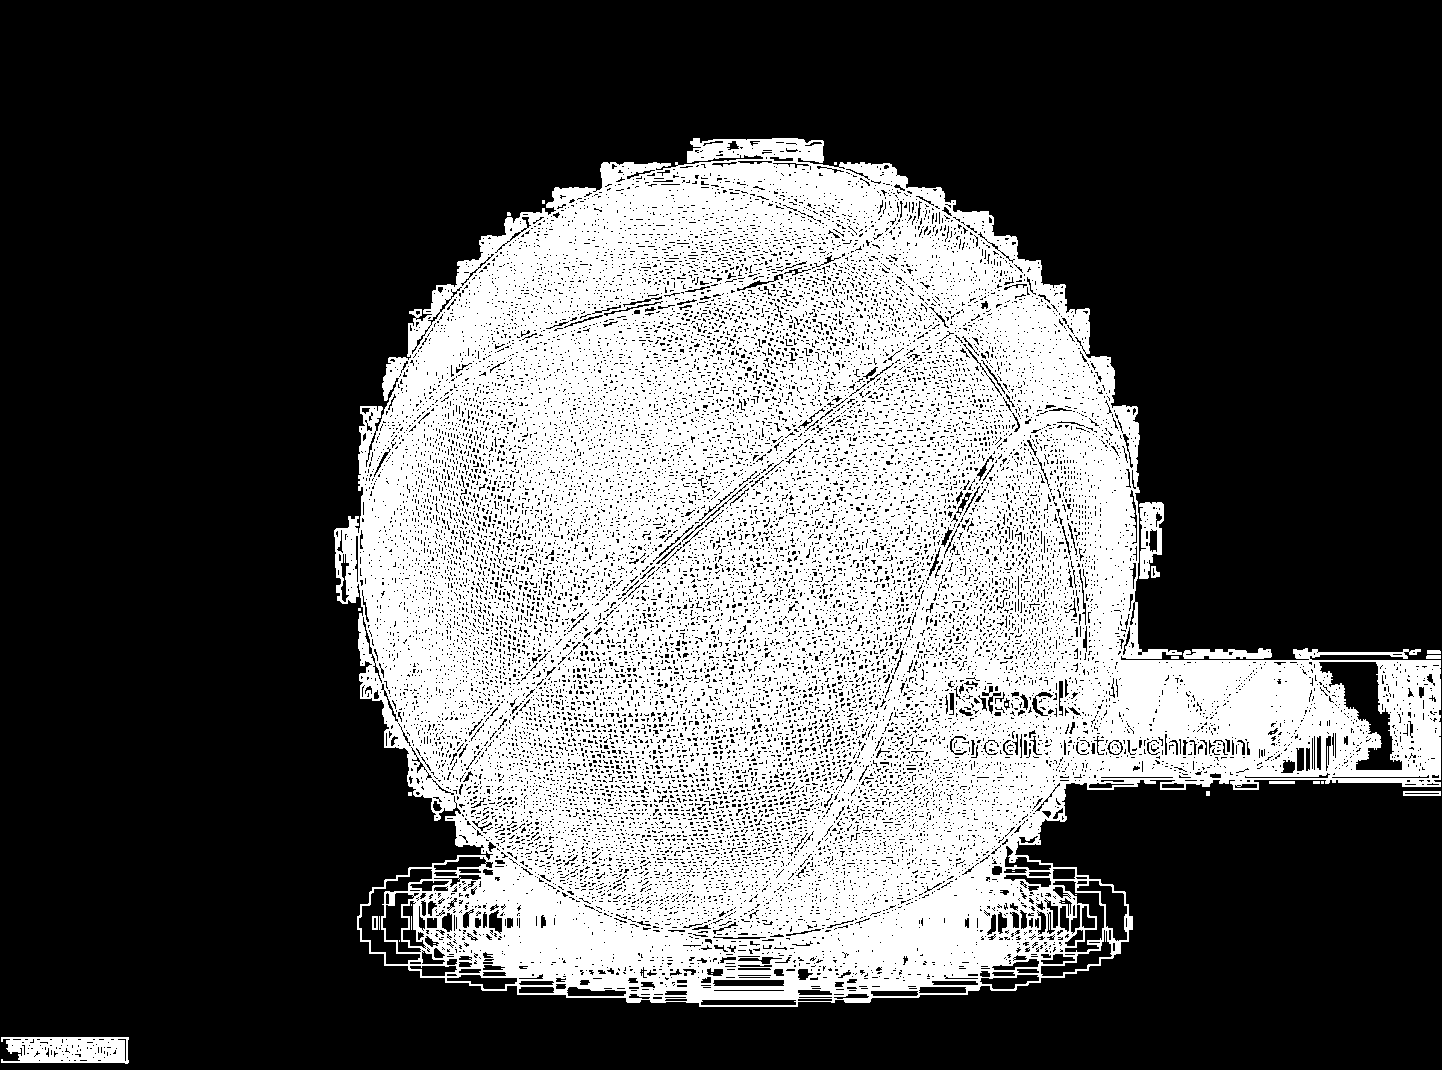
\includegraphics[width=\linewidth]{log.png}
    \caption{Εικόνα μπάλας μπάσκετ με εφαρμογή \en LoG \gr.}
\end{minipage}
\hfill
\begin{minipage}{0.48\textwidth}
    \centering
    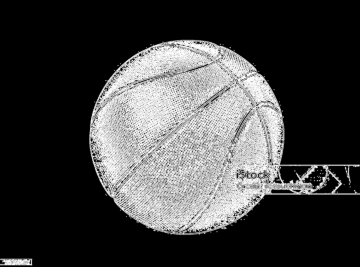
\includegraphics[width=\linewidth]{log_small.png}
    \caption{Εικόνα μπάλας μπάσκετ με εφαρμογή \en LoG \gr μειωμένης διάστασης \en pixel\gr.}
\end{minipage}

\end{figure}


\vspace{0.3cm}

\section*{Κύρια συνάρτηση \en circ\_hough()\gr}

Η συνάρτηση \en \texttt{circ\_hough()} \gr ενσωματώνει την πλήρη διαδικασία εντοπισμού κύκλων:

\begin{tcolorbox}[colback=gray!5!white, colframe=black!75!black, title=Ψευδοκώδικας \en circ\_hough()\gr]
\en
\begin{verbatim}
1. Set parameters: R_min, delta_r, num_thetas
   bin_threshold ← V_min / num_thetas

2. Convert image to grayscale if needed
3. Apply Canny edge detector

4. Call find_hough_circles(...) to extract circles

5. Save result with circles drawn
6. Extract and return centers and radii of circles
\end{verbatim}
\gr
\end{tcolorbox}

\hspace{-0.6cm}Η έξοδος αποθηκεύεται είτε ως \en \texttt{circles\_img\_sobel.png} \gr είτε \en \texttt{circles\_img\_log.png}\gr, ανάλογα με τον χάρτη ακμών που χρησιμοποιήθηκε.

\vspace{0.3cm}

\section*{Ανίχνευση κύκλων: Συνάρτηση \en find\_hough\_circles()\gr}

Αυτή είναι η «καρδιά» της μεθόδου. Πραγματοποιεί την ψήφιση για κύκλους μέσω μιας βελτιστοποιημένης λίστας πιθανών παραμέτρων.

\begin{tcolorbox}[colback=gray!5!white, colframe=black!75!black, title=Ψευδοκώδικας \en find\_hough\_circles()\gr]
\en
\begin{verbatim}
1. Prepare theta and radius ranges
2. For each edge pixel (x, y):
   - For each candidate (r, dx, dy):
       - Compute center (xc, yc) = (x - dx, y - dy)
       - Accumulate votes in (xc, yc, r)

3. Collect all entries with votes ≥ bin_threshold
4. Optionally sort by vote count and keep top_k

5. Post-process to eliminate near-duplicate circles
6. Draw circles on output image
7. Return image and list of circles
\end{verbatim}
\gr
\end{tcolorbox}

\vspace{0.3cm}

\section*{Ανάλυση εξόδου και σύγκριση}

Η συνάρτηση \en \texttt{circ\_hough()} \gr εφαρμόστηκε σε δύο χάρτες ακμών:

\begin{itemize}
    \item \textbf{\en Sobel edge map\gr:} Απλός και γρήγορος, αλλά ευαίσθητος σε θόρυβο.
    \item \textbf{\en LoG edge map\gr:} Παρέχει πιο σαφείς και ομαλές ακμές, βελτιώνοντας την ακρίβεια του εντοπισμού.
\end{itemize}

\hspace{-0.6cm}Αναλόγως με την παράμετρο \en \texttt{V\_min}\gr, ο αλγόριθμος ανίχνευσε είτε πολύ λίγους είτε πολλούς κύκλους. Η τελική επιλογή στο \en \texttt{V\_min = 40} \gr απέδωσε το περίγραμμα της μπάλας με ικανοποιητική ακρίβεια.

\vspace{0.3cm}

\section*{Εντοπισμένοι κύκλοι σε εικόνες \en log\_small, sobel\_small \gr}

Παρακάτω παρατίθενται τα αποτελέσματα που έγιναν \en demonstrate \gr στο αρχείο \en demo.py \gr υπό την κλήση της \en circ\_hough() \gr και αποθηκεύονται στον κώδικα σε μορφή \en .png\gr.

\begin{figure}[H]
\centering
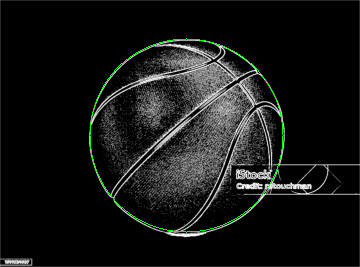
\includegraphics[width=0.6\textwidth]{circles_img_sobel.png}
\caption{Ανίχνευση κύκλων με χρήση χάρτη ακμών \en Sobel \gr. Ο εξωτερικός κύκλος εντοπίστηκε με επιτυχία.}
\end{figure}

\begin{figure}[H]
\centering
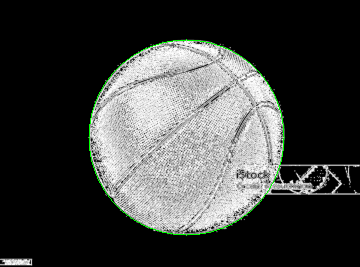
\includegraphics[width=0.6\textwidth]{circles_img_log.png}
\caption{Ανίχνευση κύκλων με χρήση χάρτη ακμών \en LoG \gr. Εντοπίζονται πολλαπλά επίπεδα περιγραμμάτων.}
\end{figure}

\vspace{0.3cm}

\section*{Συμπεράσματα και σχόλια}

Σε αυτό το σημείο θεωρώ θεμιτώ να κάνω μία επίδειξη των παραμέτρων που υπέστη \en tuning \gr προκειμένου να έχουμε τα βέλτιστα αποτελέσματα και για τις δύο περιπτώσεις όπως αναδείχθηκαν και στο παραπάνω \en section\gr.

\vspace{0.3cm}

\hspace{-0.6cm}Συγκεκριμένα:
\begin{table}[H]
\centering
\caption{Παράμετροι για τη συνάρτηση \en \texttt{circ\_hough()}\gr}
\begin{tabular}{|c|c|p{8cm}|}
\hline
\textbf{Παράμετρος} & \textbf{Τιμή} & \textbf{Περιγραφή} \\
\hline
\en \texttt{R\_min} \gr & 95 & Ελάχιστη ακτίνα κύκλου προς ανίχνευση \\
\hline
\en \texttt{R\_max} \gr & 200 & Μέγιστη ακτίνα κύκλου προς ανίχνευση \\
\hline
\en \texttt{delta\_r} \gr & 1 & Βήμα αύξησης της ακτίνας ανά κύκλο \\
\hline
\en \texttt{num\_thetas} \gr & 100 & Αριθμός διακριτών γωνιών ανά κύκλο (360° / 100 = 3.6° ανά βήμα) \\
\hline
\en \texttt{V\_min} \gr & 40 & Ελάχιστος αριθμός ψήφων \en (votes) \gr που πρέπει να λάβει ένας κύκλος για να θεωρηθεί έγκυρος \\
\hline
\en \texttt{bin\_threshold} \gr & 0.40 & Κατώφλι ψήφων ανά αριθμό γωνιών: $V_{min} / num\_thetas$ \\
\hline
\en \texttt{min\_edge\_threshold} \gr & 100 & Κατώτερο όριο για \en edge detection \gr με \en \texttt{Canny} \gr \\
\hline
\en \texttt{max\_edge\_threshold} \gr & 200 & Ανώτερο όριο για \en \texttt{Canny edge detector} \gr \\
\hline
\en \texttt{resize scale} \gr & $1/4$ & Κλίμακα σμίκρυνσης της εικόνας πριν την εφαρμογή του \en Hough \gr για μείωση του κόστους \\
\hline
\en \texttt{top\_k} \gr & 20 & Μέγιστος αριθμός κύκλων που θα διατηρηθούν βάσει ψήφων \\
\hline
\end{tabular}
\end{table}


\vspace{0.3cm}
 
\noindent Τέλος, έχοντας και τα αποτελέσματα οπτικοποίησης εύκολα απορρέει το συμπέρασμα:

\begin{itemize}
    \item Η εφαρμογή της \en \texttt{circ\_hough()} \gr στον \en Sobel edge map \gr οδήγησε σε επιτυχή, αλλά περιορισμένη ανίχνευση κύκλων (λόγω και του \en \texttt{R\_min} \gr που έθεσα και του \en V\_min \gr) — εντοπίστηκε μόνο ο εξωτερικός κύκλος.

    \item Η εφαρμογή της ίδιας συνάρτησης στον \en LoG edge map \gr παρείχε περισσότερους κύκλους, περιγράφοντας με μεγαλύτερη λεπτομέρεια τα εσωτερικά χαρακτηριστικά του αντικειμένου ωστόσο και πάλι με κατάλληλη επιλογή παραμέτρων καταφέραμε να αναδείξουμε τον μοναδικό κύκλο που περιβάλλει την μπάλα.
    
    \item Η χρήση \en LoG \gr συνεπώς προσφέρει περισσότερες πληροφορίες, αλλά ενδέχεται να προσθέσει και παραπανίσιες ανιχνεύσεις, ανάλογα με τις παραμέτρους που θα οριστούν για μεγαλύτερη ελευθερία ανίχνευσης. Αντίθετα, ο \en Sobel \gr είναι πιο στοχευμένος και φιλτραρισμένος — κατάλληλος για ανίχνευση κυρίως έντονων ορίων. Ωστόσο, με τις παραμέτρους που έθεσα, εντοπίζεται σωστά η σφαίρα ως μοναδικός κύκλος.

    \item Η ποιότητα της εξαγόμενης πληροφορίας εξαρτάται τόσο από την επιλογή του \en edge detector \gr όσο και από την παράμετρο \en \texttt{V\_min} \gr που φιλτράρει τους υποψήφιους κύκλους.
\end{itemize}

\hspace{-0.6cm}Ο κώδικας βρίσκεται στο \en \texttt{circ\_hough.py} \gr και η υλοποίηση του κυκλικού μετασχηματισμού στο \en \texttt{find\_hough\_circles()}\gr.

\bibliographystyle{plain}
\begin{thebibliography}{1}
    \bibitem{lnmpikas}
    \en https://numpy.org/doc/
    \bibitem{psee}
    \en https://docs.opencv.org/4.x/index.html
    \bibitem{circ_hough_opencv}
    \en https://docs.opencv.org/3.4/d4/d70/tutorial\_hough\_circle.html
    \bibitem{circ_hough_docs}
    \en https://en.wikipedia.org/wiki/Circle\_Hough\_Transform
\end{thebibliography}

\end{document}